\section{Data Pre-processing}
\label{sec:data}
% \dq{@Da Shi}

% \subsection{Data Overview}
% \dq{@tigerhu @easonfanfan @jamesjzhou @jodai}

% Our pre-training dataset comprises approximately 210 million diverse video-text pairs and roughly 2.5 billion image-text pairs. 
We use an image-video joint training strategy.
The videos are meticulously divided into five distinct groups, while images are categorized into two groups, each tailored to fit the specific requirements of their respective training processes. This section will primarily delve into the intricacies of video data curation.

% The origins of our data are diverse, encompassing open-source datasets, data supply companies, data trading markets, and various other data proprietors. 
% Given the substantial volume and intricate origins of the data, it is crucial to ensure strict adherence to legal regulations concerning data privacy, data protection, and intellectual property rights. 
Our data acquisition process is rigorously governed by the principles outlined in the General Data Protection Regulation (GDPR) \cite{investopedia_gdpr} framework. Furthermore, we employ advanced techniques such as data synthesis and privacy computing to guarantee compliance with these stringent standards.

Our raw data pool initially comprised videos spanning a wide range of domains including people, animals, plants, landscapes, vehicles, objects, buildings, and animation. Each video was acquired with a set of basic thresholds, including minimum duration requirements. Additionally, a subset of the data was collected based on more stringent criteria, such as spatial quality, adherence to a specific aspect ratio, and professional standards in composition, color, and exposure. These rigorous standards ensure that our videos possess technical quality and aesthetic appeal. We experimentally verified that incorporating high-quality data is instrumental in significantly enhancing model performance.


\begin{figure}[t]
    \centering
    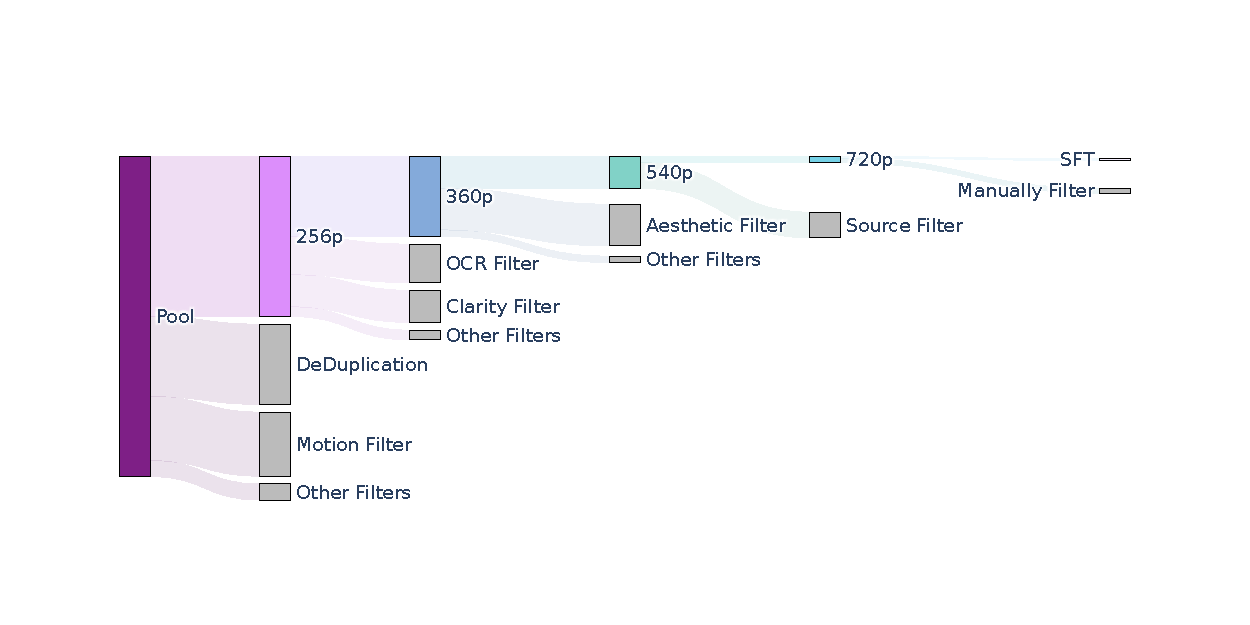
\includegraphics[trim=1cm 2cm 2cm 1cm,width=\linewidth]{figures/video-data-curation.pdf}
     \caption{
     \textbf{Our hierarchical data filtering pipeline.} 
     We employ various filters for data filtering and progressively increase their thresholds to build 4 training datasets, i.e., 256p, 360p, 540p, and 720p, while the final SFT dataset is built through manual annotation. This figure highlights some of the most important filters to use at each stage. A large portion of data will be removed at each stage, ranging from half to one-fifth of the data from the previous stage. 
     Here, gray bars represent the amount of data filtered out by each filter while colored bars indicate the amount of remaining data at each stage.
     }
    \label{fig:video-data-curation}
\end{figure}


\subsection{Data Filtering}
\label{data_filtering}
% \dq{@jamesjzhou @jodai @junkun}

Our raw data from different sources exhibits varying durations and levels of quality. To address this, we employ a series of techniques to pre-process the raw data. Firstly, we utilize PySceneDetect~\cite{pyscene} to split raw videos into single-shot video clips. Next, we employ the Laplacian operator from OpenCV~\cite{opencv} to identify a clear frame, serving as the starting frame of each video clip. Using an internal VideoCLIP model, we calculate embeddings for these video clips. These embeddings serve two purposes: (i) we deduplicate similar clips based on the Cosine distance of their embeddings; (ii) we apply k-means~\cite{macqueen1967some} to obtain $\sim$10K concept centroids for concept resampling and balancing.

To continuously enhance video aesthetics, motion, and concept range, we implement a hierarchical data filtering pipeline for constructing training datasets, as shown in Figure~\ref{fig:video-data-curation}. This pipeline incorporates various \textit{filters} to help us filter data from different perspectives which we introduce next. 
% \jd{The effects of these filters and their corresponding thresholds are validated with data selection experiments on smaller scale model.} 

We employ Dover~\cite{wu2023exploring} to assess the visual aesthetics of video clips from both aesthetic and technical viewpoints. Additionally, we train a model to determine clarity and eliminate video clips with visual blurs. By predicting the motion speed of videos using estimated optical flow~\cite{opencv}, we filter out static or slow-motion videos. We combine the results from PySceneDetect~\cite{pyscene} and Transnet v2~\cite{souvcek2020transnet} to get scene boundary information. We utilize an internal OCR model to remove video clips with excessive text, as well as to locate and crop subtitles. We also develop YOLOX~\cite{ge2021yolox}-like visual models to detect and remove some occluded or sensitive information such as watermarks, borders, and logos. To assess the effectiveness of these filters, we perform simple experiments using a smaller \nameofmethod{} model and observe the performance changes. The results obtained from these experiments play an important role in guiding the building of our data filtering pipeline, which is introduced next.

Our hierarchical data filtering pipeline for video data yields five training datasets, corresponding to the five training stages (Section ~\ref{model-pretrain}). These datasets (except for the last fine-tuning dataset) are curated by progressively improving the thresholds of the aforementioned filters. The video spatial resolution increases progressively from 256 $\times$ 256 $\times$ 65 to 720$\times$1280 $\times$ 129.
%
% Initially, our video pool contains $\sim$500M diverse video clip-text pairs. We filter out videos with height or width lower than 256 pixels and apply relatively relaxed thresholds to them, yielding the first dataset (256p) with a size of $\sim$210M. We gradually increase the resolution and filtering thresholds, leading to the second (360p), the third (540p), and the fourth (720p) training datasets with sizes of $\sim$46M, $\sim$21M, and $\sim$4M, respectively. 
%
We apply varying levels of strictness to the filters during the threshold adjustment process at different stages (see Figure~\ref{fig:video-data-curation}). The last dataset used for fine-tuning is described next. 

To improve the model's performance in the final stage (Section~\ref{sft}), we build a fine-tuning dataset comprising $\sim$1M samples. This dataset is meticulously curated through human annotation. Annotators are assigned the task of identifying video clips that exhibit high visual aesthetics and compelling content motion. Each video clip undergoes evaluation based on two perspectives: (i) decomposed aesthetical views, including color harmony, lighting, object emphasis, and spatial layout; (ii) decomposed motion views, encompassing motion speed, action integrity, and motion blurs. Finally, our fine-tuning dataset consists of visually appealing video clips with intricate motion details.

We also establish a hierarchical data filtering pipeline for images by reusing most of the filters, excluding the motion-related ones. Similarly, we build two image training datasets by progressively increasing the filtering thresholds applied to an image pool of billions of image-text pairs. 
%
The first dataset contains billions of samples and is used for the initial stage of text-to-image pre-training. The second dataset contains hundreds of millions of samples and is utilized for the second stage of text-to-image pre-training.

\subsection{Data Annotation}
% \dq{@lixin}

\textbf{Structured Captioning}. As evidenced in research \cite{videoworldsimulators2024,betker2023improving}, the precision and comprehensiveness of captions play a crucial role in improving the prompt following ability and output quality of generative models. Most previous work focus on providing either brief captions \cite{Chen_2024,li2022blip} or dense captions \cite{yang2024cogvideox,chen2023sharegpt4v,chen2024sharegpt4video}. However, these approaches are not without shortcomings, suffering from incomplete information, redundant discourse and inaccuracies. In pursuit of achieving captions with higher comprehensiveness, information density and accuracy, we develop and implement an in-house Vision Language Model(VLM) designed to generate structured captions for images and videos. These structured captions, formatted in JSON, provide multi-dimensional descriptive information from various perspectives, including: 1) \textbf{Short Description}: Capturing the main content of the scene. 2) \textbf{Dense Description}: Detailing the scene's content, which notably includes scene transitions and camera movements that are integrated with the visual content, such as camera follows some subject. 3) \textbf{Background}: Describing the environment in which the subject is situated. 4) \textbf{Style}: Characterizing the style of the video, such as documentary, cinematic, realistic, or sci-fi. 5) \textbf{Shot Type}: Identifying the type of video shot that highlights or emphasizes specific visual content, such as aerial shot, close-up shot, medium shot, or long shot. 6) \textbf{Lighting}: Describing the lighting conditions of the video. 7) \textbf{Atmosphere}: Conveying the atmosphere of the video, such as cozy, tense, or mysterious.

Moreover, we extend the JSON structure to  incorporate additional metadata-derived elements, including source tags, quality tags, and other pertinent tags from meta information of images and videos. Through the implementation of a carefully designed dropout mechanism coupled with permutation and combination strategies, we synthesize captions diverse in length and pattern by assembling these multi-dimensional descriptions for each image and video, aiming to improve the generalization ability of generative models and prevent overfitting. We utilize this captioner to provide structured captions for all images and videos in our training dataset.

\textbf{Camera Movement Types}. We also train a camera movement classifier capable of predicting 14 distinct camera movement types, including zoom in, zoom out, pan up, pan down, pan left, pan right, tilt up, tilt down, tilt left, tilt right, around left, around right, static shot and handheld shot. High-confidence predictions of camera movement types are integrated into the JSON-formatted structured captions, to enable camera movement control ability of generative models.

% \dq{Move to other chapter?}

